\section{Schema and Normalization}
\label{sec:schema}

The relational design has three domains and 22 tables. The ER/EER diagram
in Figure \ref{fig:eer} shows the full schema; primary keys are underlined
and foreign keys are rendered as directed edges. The normalization journey
is documented in detail in \texttt{docs/schema/normalization\_raw\_to\_3nf.md}
and the relation catalog in \texttt{docs/schema/data\_model\_3nf.md}; this
section summarizes the design rationale.

\begin{figure*}[htbp]
  \centering
  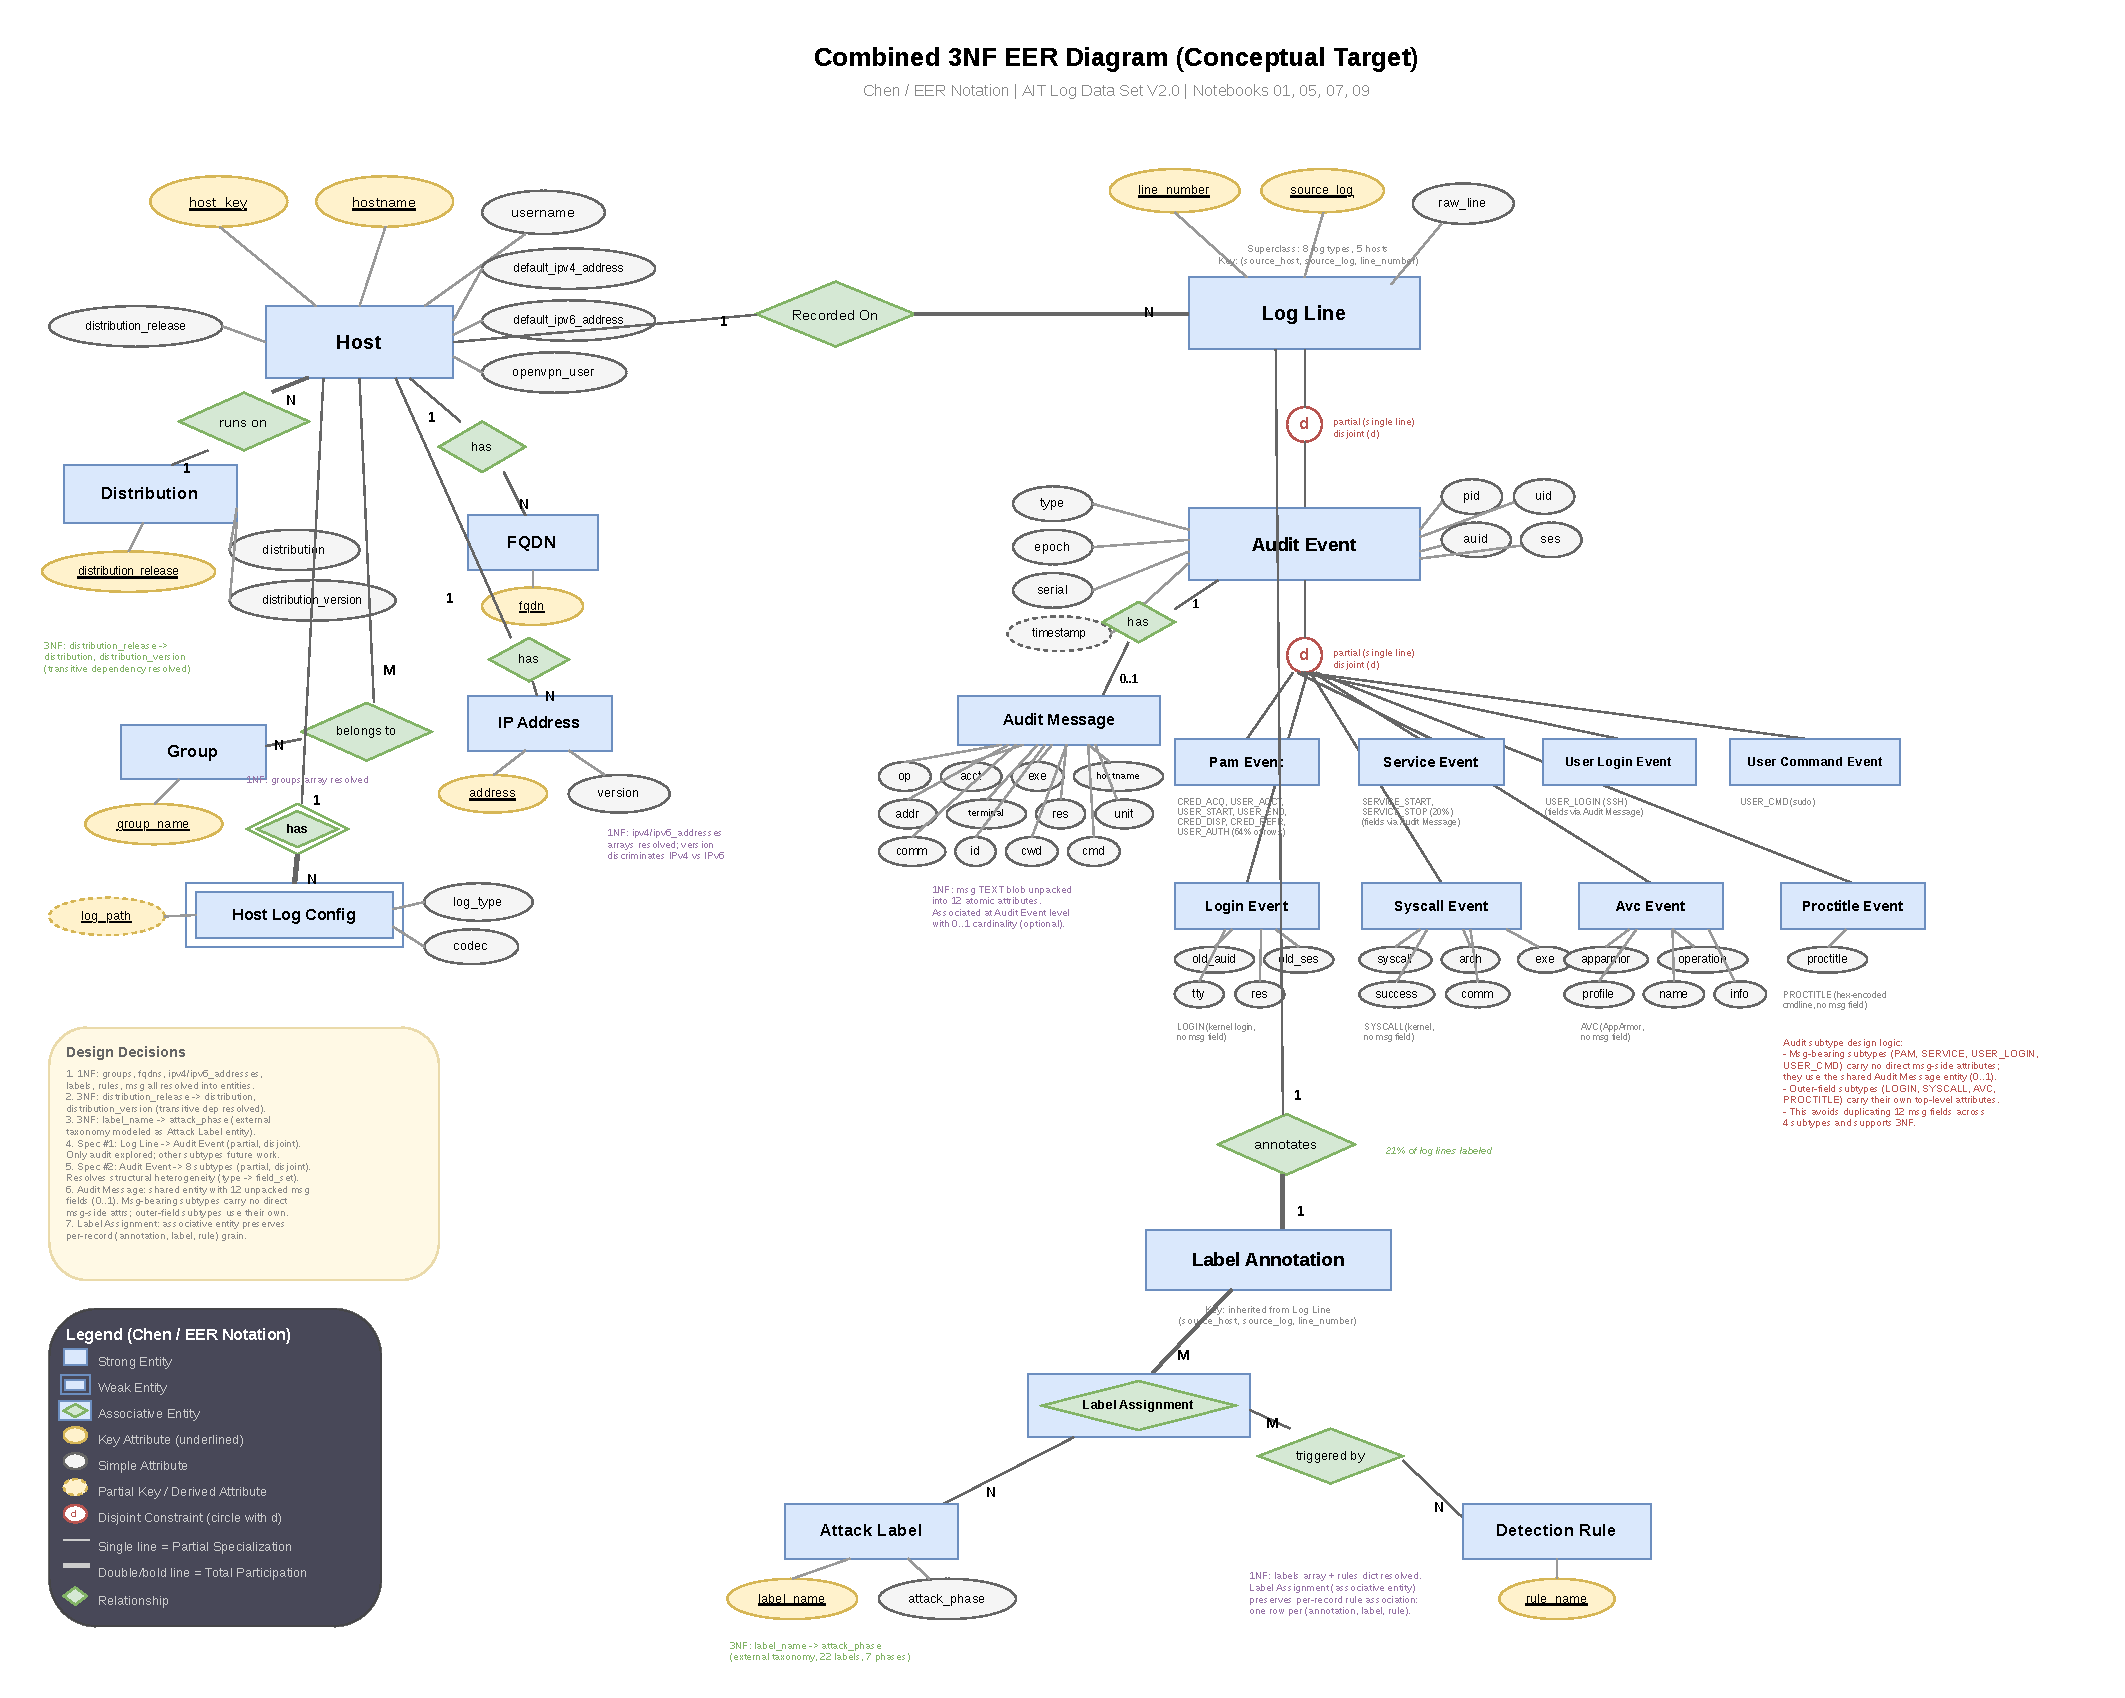
\includegraphics[width=0.95\textwidth]{figures/eer_3nf_combined.pdf}
  \caption{Final 3NF EER schema: 22 tables across host inventory (7),
    audit events (10), and attack labels (5) domains. Surrogate primary
    keys (SERIAL) are used throughout to keep foreign-key columns narrow
    across the join graph.}
  \label{fig:eer}
\end{figure*}

\subsection{Domain 1: Host Inventory (7 tables)}
The host domain captures the testbed inventory. The core entity is
\texttt{host}, with row grain ``one row per machine'' and 22 rows total.
Three multi-valued attributes (\texttt{groups}, \texttt{fqdns},
\texttt{ipv4\_addresses}, \texttt{ipv6\_addresses}) become 1NF child
tables (\texttt{host\_group}, \texttt{host\_fqdn}, \texttt{host\_ipv4},
\texttt{host\_ipv6}) with composite primary keys. The transitive
dependency
\texttt{distribution\_release} $\rightarrow$
\{\texttt{distribution}, \texttt{distribution\_version}\}
is removed by the 3NF lookup table \texttt{os\_release} (2 rows: bionic
and stretch). The \texttt{logs} composite multi-valued field becomes
\texttt{host\_log\_config} (66 rows, 1 to 9 configs per host).

\subsection{Domain 2: Audit Events (10 tables)}
The audit domain demonstrates supertype/subtype decomposition. The
supertype \texttt{audit\_event} (3{,}048 rows) carries the attributes
common to every \texttt{auditd} record (\texttt{event\_id},
\texttt{host\_id}, \texttt{type}, \texttt{epoch}, \texttt{timestamp},
\texttt{pid}, \texttt{uid}, \texttt{auid}, \texttt{ses},
\texttt{line\_number}, \texttt{raw\_line}). Two classes of subtypes
extend it:

\begin{itemize}
  \item \textbf{Msg-bearing subtypes}: \texttt{audit\_pam\_event},
    \texttt{audit\_service\_event}, \texttt{audit\_user\_login\_event},
    \texttt{audit\_user\_cmd\_event}. The semantic content for these
    subtypes lives inside the \texttt{msg=` ... '} key-value blob in the
    raw line. We resolve this 1NF violation by parsing the blob into 12
    atomic columns in \texttt{audit\_message} (2{,}614 rows), which holds
    a 0..1 relationship with \texttt{audit\_event}.
  \item \textbf{Outer-field subtypes}: \texttt{audit\_login\_event},
    \texttt{audit\_syscall\_event}, \texttt{audit\_avc\_event},
    \texttt{audit\_proctitle\_event}. These record types carry their
    semantic content as top-level fields rather than inside \texttt{msg};
    the subtype tables hold those fields directly.
\end{itemize}

The decomposition turns a hypothetical flat ``audit\_line'' table with
$\sim 44$ columns and 80\% NULL density into a supertype + 9 sparse
subtype tables with full population per subtype. The cost is more joins
in queries; the benefit is correct cardinality, query-planner statistics,
and a cleaner mental model.

\subsection{Domain 3: Attack Labels (5 tables)}
The label domain links log lines to attacker activity. The grain is one
row per \emph{labeled} log line, identified by the natural key
(\texttt{source\_host}, \texttt{source\_log}, \texttt{line\_number}).
\texttt{labeled\_line} (61{,}862 rows) is the line-level fact table;
\texttt{labeled\_line\_label} is the M:N junction connecting lines to
labels; \texttt{labeled\_line\_rule} captures which detection rule
generated each label (an event can be labeled by multiple rules). The
taxonomy is normalized into two lookup tables: \texttt{attack\_label}
(22 rows: distinct label names) and \texttt{attack\_phase} (7 rows:
kill-chain phases), with a 1:N relationship from phase to label.

\subsection{Normalization Decisions Worth Calling Out}
Three decisions are explicit project rules rather than mechanical
applications of the normalization algorithm:
\begin{enumerate}
  \item \textbf{Surrogate keys throughout.} Every entity has a SERIAL
    primary key, even when the natural key (e.g. \texttt{host\_key},
    \texttt{(source\_host, source\_log, line\_number)}) is unique. This
    keeps foreign-key columns narrow (\texttt{INT} rather than
    \texttt{VARCHAR(50)}) and decouples domain-key changes from join
    indexes. The natural key is preserved as a \texttt{UNIQUE} constraint.
  \item \textbf{Provenance preserved on the supertype.}
    \texttt{audit\_event} carries the original \texttt{raw\_line} TEXT
    even after the parsed columns are populated. This is a deliberate
    space cost in exchange for reproducibility: we can re-derive any
    parsed field from the raw text if a downstream bug is found.
  \item \textbf{One pragmatic 1NF exception.} \texttt{host\_log\_config}
    has an \texttt{add\_field\_json TEXT} column that retains the JSON
    payload of optional log-specific fields. Rather than create a
    polymorphic child table per log type (high schema cost, low query
    value), we leave the JSON opaque and query it with PostgreSQL
    \texttt{jsonb\_path\_query} when needed. The exception is documented
    and the column is unused by the queries in Section \ref{sec:sql}.
\end{enumerate}

\subsection{3NF Claim}
For each non-key attribute in every relation, we verified that the
attribute depends only on the primary key (no partial dependencies, as
all primary keys are atomic SERIAL surrogates) and that it does not
transitively depend on another non-key attribute. The two textbook
candidates for transitive dependency in the source data
(\texttt{distribution\_release} $\rightarrow$ \texttt{distribution},
\texttt{distribution\_version}) and the lookup-style relationship
(\texttt{label\_name} $\rightarrow$ \texttt{phase\_name}) are removed
by promoting them into separate lookup tables (\texttt{os\_release}
and \texttt{attack\_phase}, respectively). The one
documented exception is \texttt{host\_log\_config.add\_field\_json},
which is a TEXT blob carrying log-type-specific configuration values.
We treat the column as opaque (queried only with PostgreSQL JSON
functions when needed) rather than synthesizing a polymorphic child
table. The exception is documented in
\texttt{docs/schema/data\_model\_3nf.md} and the column is unused by
any query in Section~\ref{sec:sql}.
